% This is samplepaper.tex, a sample chapter demonstrating the
% LLNCS macro package for Springer Computer Science proceedings;
% Version 2.20 of 2017/10/04
%
\documentclass[runningheads]{llncs}
%
\usepackage[utf8]{inputenc}
\usepackage{graphicx}
\usepackage[british]{babel}
%\usepackage[backend=biber]{biblatex}
%\usepackage[backend=biber,style=splncs04]{biblatex}  %backend=biber is 'better'  

% Used for displaying a sample figure. If possible, figure files should
% be included in EPS format.
%
% If you use the hyperref package, please uncomment the following line
% to display URLs in blue roman font according to Springer's eBook style:
% \renewcommand\UrlFont{\color{blue}\rmfamily}

% ---- Bibliography ----
%
% BibTeX users should specify bibliography style 'splncs04'.
% References will then be sorted and formatted in the correct style.
%

\bibliographystyle{splncs04}
\begin{document}
%
\title{Contribution Title\thanks{Supported by organization x.}}
%
%\titlerunning{Abbreviated paper title}
% If the paper title is too long for the running head, you can set
% an abbreviated paper title here
%
\author{Maurus K\"uhne\inst{1}\orcidID{0000-0002-4205-3552} \and
Beat Tödtli\inst{2}\orcidID{0000-0003-3674-2340}} %\and
%Third Author\inst{3}\orcidID{2222--3333-4444-5555}}
%
\authorrunning{M. Kühne and B.Tödtli}
% First names are abbreviated in the running head.
% If there are more than two authors, 'et al.' is used.
%
\institute{Fernfachhochschule Schweiz\\
\url{ffhs.ch}\and
Institut für Informations- und Prozessmanagement, FHS St.Gallen, \\
\email{beat.toedtli@ost.ch}\\
\url{fhsg.ch} 
}
%
\maketitle              % typeset the header of the contribution
%
\begin{abstract}
The abstract should briefly summarize the contents of the paper in
150--250 words.
\cite{yu_generating_2018}
\keywords{First keyword  \and Second keyword \and Another keyword.}
\end{abstract}
%
%
%
\subsection{Introduction}
The discovery of Szegedy et.al.~\cite{Szegedy_2014} that several machine learning models, including deep neural networks are vulnerable to \emph{adversarial attacks} was seminal for a new subfield of studying deep learning. Probably the most intriguing, but also unsettling result was that adversarial examples can be made quite imperceptible to the human eye, while still fooling a convolutional neural network to misclassify the image~\cite{goodfellow_2014}. Subsequent work has developed various attack algorithms in a variety of black-box, gray-box and white-box scenarios as well as defensive strategies such as adversarial training~\cite{REN2020346}. In particular Moosavi-Dezfooli et.al. have demonstrated~\cite{moosavi-dezfooli_universal_2017} that the perturbations can be \emph{universal}, i.e. that a single set of of pixel value changes can be found that fools a network on a large fraction of the training data set. Moreover, these \emph{universal perturbations} also fool other convolutional networks, albeit to a lesser but still very significant degree~{\bf cite universal adversarial attacks}. 
Given these results it seems plausible that neural networks partly share a common structure that can be expoited by universal adversarial perturbations, while yet other aspects are different. In this context, we ask whether the transferability of universal adversarial perturbations to new convolutional neural networks is improved by combining two neural networks in the adversarial perturbation generation algorithm. We expect to see an increase in the transferability of an adversarial perturbation to new networks by combining two neural networks. Ultimately, we hope this approach could lead to identifying a general property resulting in convolutional neural networks being susceptible ({\bf sensitive?} to adversarial attacks.

Given the practical potential and relevance of Deep Learning and the above potential security threats, finding a robust resolution is important and urgent. However, research into the topic is hampered by the \emph{reproducibility crisis} in machine learning~\cite{raff2020quantifying}. A lot of research results, including on adversarial attacks, remain poorly documented in publications. While the methods described may be general enough to be useful for many similar applications, 
the published results may not be reproducible due to undocumented values for hyperparameters, software library versions etc.

ev https://arxiv.org/vc/arxiv/papers/1909/1909.03032v1.pdf zitieren?

Also, only in rare cases is it clear how well the published results generalize beyond the very specific data set that was used but not provided to produce the published results. 

While not being able to reproduce the generation of adversarial examples may seem beneficial at first sight, it is clear that a thorough resolution of such security issues requires a well-stated problem including readily available state-of-the-art algorithms for the production of adversarial examples. They form the basis of being able to test deep learning systems against such attacks. 

In this paper we report on an effort to reproduce results from~\cite{moosavi-dezfooli_universal_2017} {\bf und weiteren Artikeln, zitieren!} and provide our code. The authors there report good generalization results for universal adversarial perturbations across different deep learning architectures. We report on our reproduction effort and investigate whether modifications of DeepFool are able to improve the generalization capability of universal adversarial perturbations. Specifically, we ask whether adaptations in the universal adversarial example generation algorithm 
towards incorporating information from a second neural network architecture improves the fooling rate of a third neural network. ({\bf Satz zu laaang!}). 

- Introduction: adversarial perturbations sind wichtig. 
  Motivation: Vermeidung von Störbarkeit von Netzwerken
	Mozavi dezfoli: es gibt effektive universal adversarial perturbations (auf einer Netzwerkarchitektur trainiert)
	
	Verweis auf noch unbekannte Arbeit
	Fragestellung:
		- Reprodution der Resultate von Mozavi Dezfoli
		- Steigt die Transferierbarkeit von Störwerten, indem ein universal adv. pert verfahren benutzt wird, das mehrere Modelle/Netzwerke kombiniert. 
		- Wir berichten über drei Kombinationsverfahren. und vergleichen diese mit den Resultaten der Originalverfahren.
\subsection{Methods}
- Beschreibung DeepFool
- Beschreibung UAP-Verfahren: Wie werden adv. perturbations von DeepFool zu universal adv. pert. kombiniert
- Beschreibung Kombinationsverfahren: Beschreibe Verfahren ohne modifiziertes DeepFool
\subsection{Results}
\subsubsection{Versuch der Reproduktion Mozavi dezfoli}
		- Resultate Tabelle 7.3. vorstellen und diskutieren:
			- Störwerte und gestörtes Netzwerk identisch 3\%-20\% schlechter als Mozavi
			- gestörtes Netzwerk nicht identisch zum Netzwerk das Störung generiert hat: teilweise bis zu 10\% und 30\% schlechter. 
		- Resultat: Reproduktion sieht qualitativ ähnlich aus. Abb 7.1.
		- ausgeglichenes Datenset; 
		- erwähne, dass Publikation unvollständig für Reproduktion: Defaultwerte von Parameter, welche nicht in publikation beschrieben; Parameterwerte von DeepFool nicht mehr angegeben.
		- Versuch, verschiedene Parameter zu optimieren wurde versucht, brachte nur ca. 5\% Verbesserung
\subsubsection{Kombinationsverfahren}
- Tabelle	8.1 ohne Modifiziertes DeepFool
- Diskussion Resultate Reproduktion des UAP-Verfahrens: 
- Diskussion Resultate Kombinationsverfahren: kombiniere Inception und VGG, optimiere Störwerte
Vergleiche mit störwerten, die direkt auf einem einzelnen Modell generiert werden. Vergleiche einerseits mit Störwerten der Einzelmodelle, andererseits mit Störwerten eines unabhängigen Modells (ResNet)

\subsubsection{Discussion}
- Einzelne Parameter konnten nicht gut optimiert werden wegen fehlender Rechenleistung
\subsubsection{Conclusion and Outlook}
Weitere Modellpaare kombinieren.


Lorem ipsum dolor sit amet, consectetur adipiscing elit, sed do eiusmod tempor incididunt ut labore et dolore magna aliqua. Nunc sed augue lacus viverra vitae congue eu consequat. Pellentesque habitant morbi tristique senectus et. Tortor condimentum lacinia quis vel eros donec ac odio tempor. Nibh ipsum consequat nisl vel. Varius sit amet mattis vulputate enim. Ullamcorper eget nulla facilisi etiam dignissim. Sit amet est placerat in. Sed ullamcorper morbi tincidunt ornare massa eget egestas purus. Nibh nisl condimentum id venenatis a condimentum. Quisque sagittis purus sit amet volutpat consequat mauris nunc.

Aliquet risus feugiat in ante metus dictum at. Molestie nunc non blandit massa. Dignissim sodales ut eu sem integer vitae justo. Magna ac placerat vestibulum lectus mauris ultrices eros. Dolor magna eget est lorem ipsum dolor sit amet consectetur. Tincidunt tortor aliquam nulla facilisi cras fermentum odio. Gravida rutrum quisque non tellus orci ac. In vitae turpis massa sed elementum tempus egestas sed. Sit amet luctus venenatis lectus magna fringilla urna. Nibh cras pulvinar mattis nunc sed blandit libero volutpat. Blandit cursus risus at ultrices mi tempus imperdiet nulla malesuada. Non tellus orci ac auctor augue mauris augue neque gravida. Commodo sed egestas egestas fringilla phasellus faucibus scelerisque eleifend. Vitae suscipit tellus mauris a diam.

Pellentesque pulvinar pellentesque habitant morbi tristique senectus. Porttitor lacus luctus accumsan tortor posuere ac ut consequat semper. Velit egestas dui id ornare arcu odio ut sem nulla. Velit laoreet id donec ultrices tincidunt arcu non. Amet purus gravida quis blandit turpis. Malesuada fames ac turpis egestas. Pharetra convallis posuere morbi leo. Proin nibh nisl condimentum id venenatis. Diam vulputate ut pharetra sit amet. Nunc eget lorem dolor sed viverra ipsum nunc aliquet.

Leo vel fringilla est ullamcorper. Integer vitae justo eget magna fermentum iaculis eu. Mi eget mauris pharetra et ultrices. Augue ut lectus arcu bibendum at. Cursus vitae congue mauris rhoncus aenean vel elit scelerisque mauris. Vulputate odio ut enim blandit volutpat maecenas volutpat. Nisi quis eleifend quam adipiscing vitae. Imperdiet dui accumsan sit amet nulla facilisi morbi tempus iaculis. Risus in hendrerit gravida rutrum. Tempus quam pellentesque nec nam aliquam sem. Praesent tristique magna sit amet. Quam viverra orci sagittis eu volutpat odio facilisis. Nunc faucibus a pellentesque sit amet porttitor.

Amet mauris commodo quis imperdiet massa tincidunt nunc pulvinar sapien. Diam sollicitudin tempor id eu nisl nunc mi. Proin fermentum leo vel orci porta non pulvinar. Et molestie ac feugiat sed lectus vestibulum mattis ullamcorper velit. Tincidunt ornare massa eget egestas purus viverra accumsan. Amet est placerat in egestas erat imperdiet sed euismod. Turpis nunc eget lorem dolor. Volutpat sed cras ornare arcu dui vivamus. Turpis massa tincidunt dui ut ornare lectus sit. Etiam tempor orci eu lobortis elementum nibh. Dictumst vestibulum rhoncus est pellentesque elit. Duis at tellus at urna condimentum mattis pellentesque. Sollicitudin aliquam ultrices sagittis orci a scelerisque purus. Nec dui nunc mattis enim ut tellus elementum sagittis vitae. Vulputate mi sit amet mauris commodo quis imperdiet massa tincidunt.


\section{Introduction}
Moozavi-Dezfoli\cite{fawzi_robustness_2017}\\
DeepFool: a simple and accurate method to fool deep neural:\cite{moosavi-dezfooli_deepfool_2016}\\
Universal adversarial perturbations:\cite{moosavi-dezfooli_universal_2017}
\subsection{Results}
Please note that the first paragraph of a section or subsection is
not indented. The first paragraph that follows a table, figure,
equation etc. does not need an indent, either.

Subsequent paragraphs, however, are indented.

\subsubsection{Sample Heading (Third Level)} Only two levels of
headings should be numbered. Lower level headings remain unnumbered;
they are formatted as run-in headings.

\paragraph{Sample Heading (Fourth Level)}
The contribution should contain no more than four levels of
headings. Table~\ref{tab1} gives a summary of all heading levels.

\begin{table}
\caption{Table captions should be placed above the
tables.}\label{tab1}
\begin{tabular}{|l|l|l|}
\hline
Heading level &  Example & Font size and style\\
\hline
Title (centered) &  {\Large\bfseries Lecture Notes} & 14 point, bold\\
1st-level heading &  {\large\bfseries 1 Introduction} & 12 point, bold\\
2nd-level heading & {\bfseries 2.1 Printing Area} & 10 point, bold\\
3rd-level heading & {\bfseries Run-in Heading in Bold.} Text follows & 10 point, bold\\
4th-level heading & {\itshape Lowest Level Heading.} Text follows & 10 point, italic\\
\hline
\end{tabular}
\end{table}

Whenever possible, use vector graphics instead (see
Fig.~\ref{fig1}).

\begin{figure}
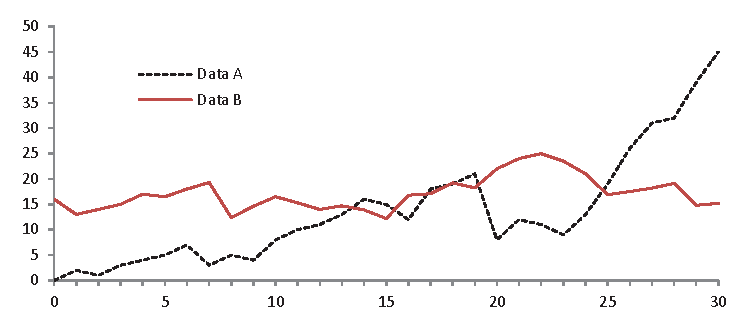
\includegraphics[width=\textwidth]{fig1.eps}
\caption{A figure caption is always placed below the illustration.
Please note that short captions are centered, while long ones are
justified by the macro package automatically.} \label{fig1}
\end{figure}


\bibliography{KuehneToedtli}

\end{document}
